\documentclass{slides}

\usepackage{tikz-uml}

\lstset{language=C++}

\begin{document}

\graphicspath{{figures/}}

\title[Object-oriented Programming]{\Large Object-oriented Programming}

\author[A. Arnold and O. Lenz]{Axel Arnold \and Olaf Lenz} 
\institute{Institut für Computerphysik\\Universit\"at Stuttgart}
\date{March 17 - 21, 2014}

\setbeamertemplate{footline}{}
\begin{frame}
  \titlepage
\end {frame}
\setbeamertemplate{footline}[icp]

\begin{frame}
  \frametitle{Outline}

  \begin{itemize}
  \item Basic ideas
  \item UML -- Universal Markup Language
  \item Classes, Interfaces and Methods
  \item Objects/Instances
  \item Composition/Fields
  \item Inheritance
  \item Polymorphism
  \end{itemize}

  \begin{block}{Literature}
    \begin{itemize}
    \item Bruce Eckels, ``Thinking in C++'', 2nd edition, Prentice-Hall
    \item Martin Fowler, ``UML Distilled'', 3rd edition, Addison-Wesley
    \end{itemize}
  \end{block}
  
\end{frame}

\begin{frame}
  \frametitle{Object-oriented Programming (OOP)}

  \begin{itemize}
  \item OO is a language-indedependent concept
  \item in principle not limited to programming (OO design)\\
    $\implies$ databases, business plans
  \item improves reusability and exchangability of code
  \item separation of partial problems
  \item ``real world'' modelling
  \item representation in \alert{Universal Markup Language} (UML)
  \end{itemize}
  \medskip

  \tikzumlset{font=\tiny}
  \begin{tikzpicture}[scale=1.1]
    \begin{umlsystem}[x=4, fill=red!10]{C++ course}
      \umlusecase{Lectures}
      \umlusecase[x=4]{Chapters}

      \umlusecase[y=-1]{Exercises}
      \umlusecase[x=4, y=-1]{Small tasks}
      \umlusecase[x=3, y=-1.7]{Project}
    \end{umlsystem}

    \umlactor[scale=0.5]{Olaf/Axel}
    \umlactor[scale=0.5,y=-1.5]{Participant}

    \umlassoc{Participant}{usecase-1}
    \umlassoc{Olaf/Axel}{usecase-1}
    \umlassoc{Participant}{usecase-3}
    \umlassoc{Olaf/Axel}{usecase-3}
    \umlinclude{usecase-1}{usecase-2}
    \umlinclude{usecase-3}{usecase-4}
    \umlinclude{usecase-3}{usecase-5}
  \end{tikzpicture}
\end{frame}

\begin{frame}
  \frametitle{Basic ideas}

  \begin{itemize}
  \item \alert{Everything is an object}\\
    \emph{Axel, students, lecture}\\
	  \emph{project, world, spy, information}
  \item \alert{Objects interact by sending/receiving messages}\\
    \emph{Axel $\rightarrow$ students: object orientation is a concept}\\
    \emph{world $\rightarrow$ map: what is the object at
      position X?}\\
  \item \alert{An object consists of objects}\\
    \emph{a course consists of lectures}\\
    \emph{a world consists of land or water fields}\\
  \item \alert{Every object has a type}\\
    \emph{Axel is a teacher}\\
    \emph{the map is a rectangle of land / water fields}
  \item \alert{All objects of the same type understand the same messages}\\
    \emph{all students hear the lecture}\\
    \emph{all spies can retrieve information}
  \end{itemize}
\end{frame}

\begin{frame}
  \frametitle{Basic ideas -- in C++}

  \begin{itemize}
  \item \alert{Everything is an object}\\
    \emph{objects are variables}\\
		~
  \item \alert{Objects interact by sending/receiving messages}\\
    \emph{methods (member functions) acting on an object (variable)}\\
    \emph{exchanged information in arguments and return values}
  \item \alert{An object consists of objects}\\
    \emph{structured objects/records}\\
    \emph{smallest units: C datatypes, int, char, ...}\\
  \item \alert{Every object has a type}\\
    \emph{classes or plain old data types in C++}\\
    \emph{types can be derived from others }
  \item \alert{All objects of the same type understand the same messages}\\
    \emph{class declaration lists member functions (messages)}\\
    \emph{member functions can be inherited}
  \end{itemize}
\end{frame}

\begin{frame}
  \frametitle{Classes, Interfaces and Methods}

  \begin{center}
    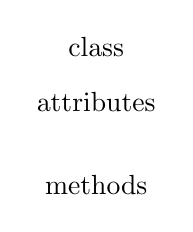
\begin{tikzpicture}[x=\textwidth,y=1em]
      \umlclass[x=0, y=0,type=abstract]{World}{
        spies : ListOfSpies
      }{
        setSpyCount(count: int)\\
        getSpyCount() : int\\[\smallskipamount]
		getMap() : Map
      }
			\draw (0.3, 3) node {\alert{class}};
			\draw (0.3, 1) node {\alert{attributes}};
			\draw (0.3, -2) node {\alert{methods}};

      \umlclass[x=0.6, y=0,type=abstract]{Map}{
        tiles: VectorOfTiles
      }{
        getWidth() : int\phantom{p}\\
        getHeight() : int\\[\smallskipamount]
        at(x: int, y:int) : Tile
      }

    \end{tikzpicture}
  \end{center}

	\begin{itemize}
    \item \alert{classes} describe the type of objects (define their \alert{interface})
    \item the interface consists of \alert{methods} and \alert{attributes} / properties
    \item methods
      \begin{itemize}
      \item are functions that operate on objects of this class
      \item can take extra arguments of arbitrary types
      \item can return values of arbitrary types
      \end{itemize}
    \item attributes are objects of arbitrary other types
  \end{itemize}
\end{frame}

\begin{frame}
  \frametitle{Objects/Instances}

  \begin{center}
    \begin{tikzpicture}[x=\textwidth]
      \begin{umlseqdiag}
      \umlobject[x=0.2,class=Map]{map}
      \umlobject[x=0.4,class=World]{world}
      \begin{umlcall}[op=width(),return=1234]{world}{map}\end{umlcall}
      \umlcreatecall[x=0.7,class={HQ},stereo=multi]{world}{headquarters}
      \umlcreatecall[x=0.7,class={Spy},stereo=multi]{world}{spy}
      \end{umlseqdiag}
    \end{tikzpicture}
  \end{center}

  \begin{itemize}
    \item every object has an immutable class assigned when it is created
    \item compare: declaration of a variable in C/C++
    \item objects communicate via their class interfaces
    \item classes can communicate  via static member functions
  \end{itemize}
\end{frame}

\begin{frame}
  \frametitle{Overloading and signature}
  
  \begin{center}
    \begin{tikzpicture}
      \umlclass[type=abstract]{Spy}{ }{
        \umlvirt{setPos(x : int, y : int)}\\
        \umlvirt{setPos(pos: Position)}
      }
    \end{tikzpicture}
  \end{center}

  \begin{itemize}
  \item a method is described by name and \alert{signature}
  \item signature is formed by the types of all taken arguments
    \begin{itemize}
    \item setPos(\emph{x : int, y : int})\\
    \item setPos(\emph{pos : Position})
    \end{itemize}
  \item methods with identical names but different arguments can exist in one class -- \alert{overloading} 
  \item return type is \emph{not} part of the signature -- cannot always resolve overload at compile time
  \item C++: constness (\lstinline[style=inline]!const!) is part of the signature
  \end{itemize}
\end{frame}

\begin{frame}
    \frametitle{Composing classes}

  \begin{center}
    \begin{tikzpicture}
      \umlclass[type=abstract]{World}{
        map : Map
      }{
        setSpyCount(count : int)\\
        getSpyCount() : int
      }

      \umlclass[x=6,type=abstract]{Spy}{
        x, y : int
      }{
        \umlvirt{setPos(x : int, y : int)}\\
        \umlvirt{setPos(pos : Position)}
      }
      \umlunicompo[mult2=*,anchors=10 and 170]{World}{Spy}
      \umluniassoc[mult2=1,anchors=-170 and -10]{Spy}{World}
    \end{tikzpicture}
  \end{center}

    \begin{itemize}
    \item objects are made of objects (\alert{attributes}) ---\\
      classes declare the types of these objects
    \item simple attributes appear below class name
    \item complex classes shown as \alert{composition}
    \item ``has-a'' or ``has-many'' relations:
      \begin{itemize}
        \item \emph{a world hosts many spies},
        \item \emph{a spy belongs to one world}
      \end{itemize}
    \end{itemize}

\end{frame}

\begin{frame}
  \frametitle{Inheritance and class hierarchy}

  \begin{center}
    \begin{tikzpicture}
      \umlclass[y=1,x=4,type=abstract]{Tile}{
        map : Map
      }{
        \umlvirt{tryStep(...)}
      }
      \umlclass{WaterTile}{
      }{
        tryStep(...)
      }

      \umlclass[x=8]{LandTile}{
      }{
        tryStep(...)
      }

      \umlinherit{WaterTile}{Tile}
      \umlinherit{LandTile}{Tile}
    \end{tikzpicture}
  \end{center}
  
  \begin{itemize}
    \item subclasses of classes -- \alert{class hierarchy}
    \item subclasses inherit methods and attributes of all superclasses
    \item no need to duplicate code
    \item .. but methods might behave differently
      (\alert{polymorphism})
      \begin{itemize}
      \item in C++: explicitely declared by keyword \lstinline![style=inline]!virtual!
    \end{itemize}
    \item \alert{abstract class}es implement only parts of the interface
      \begin{itemize}
      \item in C++: a class with purely virtual functions is abstract
      \item explicitely declared by \lstinline[style=inline]!virtual function() = 0;!
      \end{itemize}
    \end{itemize}
\end{frame}

\begin{frame}
  \frametitle{Implementation hiding}
  \tikzumlset{font=\tiny}
  \begin{center}
    \begin{tikzpicture}
      \umlclass[type=abstract]{Tile}{
        \# map : Map
      }{
        \umlvirt{+ tryStep(...)}
      }
      \umlclass[y=-2]{WaterTile}{
      }{
        + tryStep(...)
      }
      \umlclass[x=4,y=-1]{Spy}{
        - reserves : int
      }{
      }
      
      \umlinherit{WaterTile}{Tile}
      \umldep{Spy}{WaterTile}
      \umldep{Spy}{Tile}
    \end{tikzpicture}
  \end{center}

  \begin{itemize}
  \item \alert{public} (`+') elements are visible to all
  \item \alert{protected} (`\#') elements are only visible to derived classes
  \item \alert{private} (`-') attributes or methods are \emph{not} visible to
    other objects
  \item \lstinline[style=inline]!map! is protected $\implies$ visible to
    \lstinline[style=inline]!WaterTile!, not to \lstinline[style=inline]!Spy!
  \item \lstinline[style=inline]!Spy! can access \lstinline[style=inline]!tryStep! of all tiles
  \item \lstinline[style=inline]!reserves! is not visible to anybody
  \end{itemize}
\end{frame}

\end{document}
